\noindent{\Huge Narrow Phase}

Ta faza polega na dokładnym wykryciu kolizji pomiędzy obiektami i pewną odpowiedzią czy obiekty kolidują czy też nie. Obliczenia w tej fazie powinny być tak dokładne jak to możliwe.\\

\noindent{\Large Wykrywanie kolizji metodą Pixel Perfect Collission Detection}\smallskip

Ta metoda jest używana zazwyczaj w grach dwuwymiarowych, gdzie model można przedstawić w postaci siatki pikseli, na której każdy piksel ma dwa kolory, jeden przedstawiający zawieranie się danego piksela w modelu obiektu i drugi w przeciwnym przypadku, zazwyczaj czarny.

Testowanie kolizji dwóch obiektów polega na nałożeniu odpowiednio przesuniętych siatek obu obiektów na siebie i sprawdzeniu, czy istnieją piksele w których kolor obu modeli się pokrywa.

Obliczenia te można do\'sć łatwo wykonać na wielu wątkach jednocze\'snie, czasami były one też wspomagane sprzętowo. W dzisiejszych czasach to rozwiązanie jest jednak do\'sć rzadko spotykane.

Można zasymulować tą metodę przy pomocy odpowiednio napisanej funkcji rysującej modele na buforze, a następnie sprawdzeniu czy bufor zawiera piksel w danym kolorze. Możliwe jest wtedy użycie do rysowania np. karty graficznej, co znacznie przyspieszyłoby obliczenia.\bigskip

Poniżej jest napisany w pseudokodzie przykładowy algorytm sprawdzania zderzenia między dwoma obiektami.\\
Siatki składają się z pikseli, zawierających swoje położenie oraz warto\'sć, 1 je\'sli piksel należy, a 0 je\'sli nie należy do modelu.\\
Na początku algorytmu tworzony jest odpowiednio duży bufor wypełniony zerami.\\
Następnie bufor jest wypełniany jedynkami tam, gdzie pierwsza siatka ma wypełnione piksele.\\
To samo zostaje powtórzone dla drugiej siatki, z tym, że teraz zamiast ustawiać warto\'sć na 1, wykonujemy operację AND, dzięki czemu piksele będą miały warto\'sć 1 tylko tam, gdzie modele się zderzają, piksele drugiej siatki są też przesunięte.\\
Na koniec zostaje sprawdzone, czy którykolwiek z pikseli bufora ma warto\'sć 1, je\'sli tak, to zostaje zwrócona warto\'sć true, w przeciwnym wypadku zostaje zwrócona warto\'sć false.\bigskip

\noindent Obrazek \ref{pixel_perfect} ilustruje przykład użycia tej metody, pierwszy obiekt jest narysowany na czerwono, a drugi na niebiesko, miejsce zderzenia jest oznaczone przez fioletowe pola. W przypadku, gdyby nie było takich pól, oznaczałoby to, że kolizja nie zaszła.
\newpage
\begin{algorithm}[H]
	\KwIn{$m_1$ - siatka pierwszego obiektu\\ $m_2$ - siatka drugiego obiektu\\ $x, y$ - przesunięcie drugiego obiektu względem pierwszego}
	\KwOut{warto\'sć typu boolean, mówiąca czy obiekty się zderzyły czy też nie}
	\Begin{
		xMin $\leftarrow$ min(0, x);\\
		xMax $\leftarrow$ max($m_1$.width-1, $m_2$.width+x-1);\\
		yMin $\leftarrow$ min(0, y);\\
		xMax $\leftarrow$ max($m_1$.height-1, $m_2$.height+y-1);\\
		test $\leftarrow$ new ArrayOfZeroes[xMin..xMax][[yMin..yMax];\\
		\ForEach{pixel in $m_1$}{
			\If{pixel.val == 1 }{
				test[pixel.x][pixel.y] $\leftarrow$ 1;
			}			
		}
		\ForEach{pixel in $m_2$}{
			test[pixel.x][pixel.y] $\leftarrow$ test[x+pixel.x][y+pixel.y] AND pixel.val;
		}
		\ForEach{pixel in test}{
			\If{pixel == 1 }{
				return true;
			}
		}
		return false;
	}
	\caption{Algorytm wykrywający kolizję dwóch modeli metodą Pixel Perfect Collission Detection}
\end{algorithm}\bigskip
\begin{figure}[h]
	\centering
	\noindent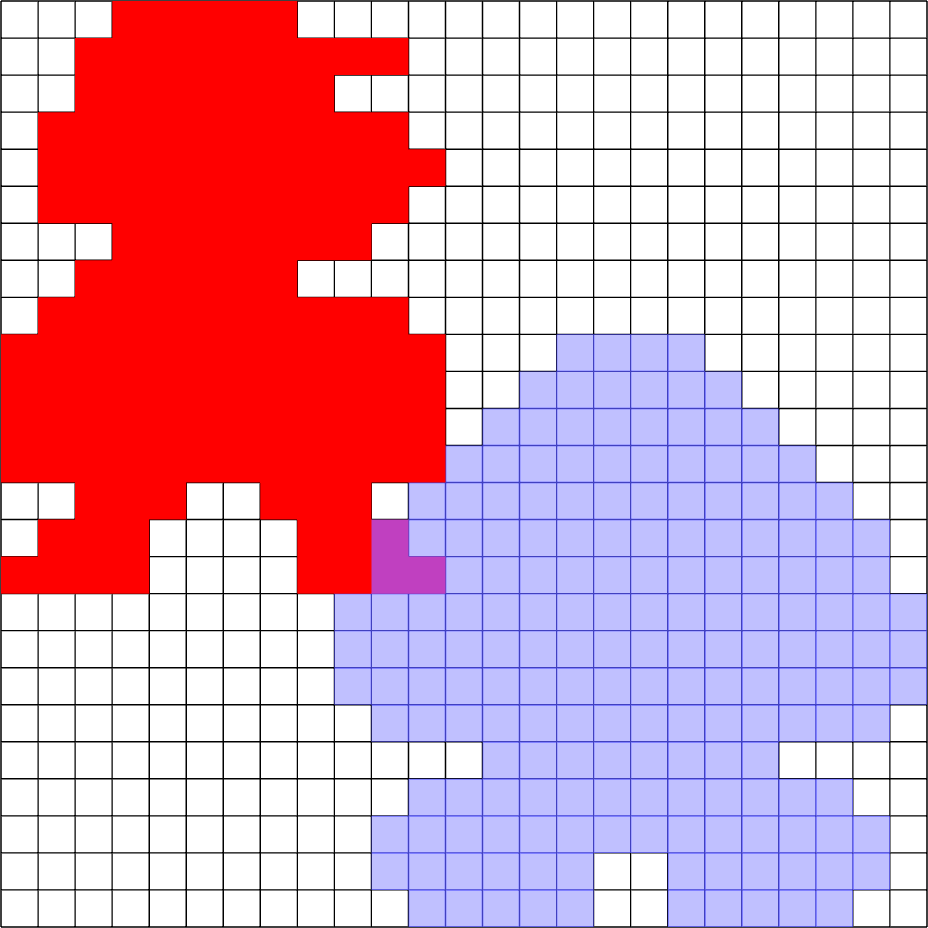
\includegraphics[width=0.65\textwidth]{collission_pixel_perfect}
	\caption{Przykład Pixel Perfect Collission Detection}
	\label{pixel_perfect}
\end{figure}
\newpage

\noindent{\Large Wykrywanie kolizji metodą Separating Planes}\smallskip

Metoda Płaszczyzn Oddzielających polega na znalezieniu płaszczyzny, która oddziela od siebie dwa obiekty.
Płaszczyzna taka istnieje je\'sli są spełnione następujące warunki:
\begin{itemize}[topsep=0.2em, itemsep=0.5em, partopsep=0em, parsep=0em]
	\item Zbiory punktów należących do obydwu obiektów są zbiorami wypukłymi
	\item Obiekty się nie pokrywają
\end{itemize}\bigskip

\noindent Zbiór wypukły to taki zbiór, w którym odcinek łączący dowolne dwa punkty ze zbioru, także znajduje się w cało\'sci w tym zbiorze.\\
Otoczka wypukła to najmniejszy zbiór wypukły, który zawiera cały dany zbiór, może być równa temu zbiorowi.\\
Aby zbiór utworzony z powierzchni danego modelu mógł być zbiorem wypukłym (czyli aby model był równy swojej otoczce wypukłej), model taki musi być wielokątem wypukłym, czyli kąt wewnętrzny między dowolnymi dwiema sąsiadującymi krawędziami musi być mniejszy lub równy $\Pi$ radianów.\\
Je\'sli modele obu zderzanych obiektów są otoczkami wypukłymi, to obiekty nie zderzają się ze sobą wtedy i tylko wtedy, gdy istnieje płaszczyzna oddzielająca te dwa modele.\\
Jednak co zrobić, gdy model nie jest równy swojej otoczce wypukłej?\\
Są na to dwa rozwiązania:
\begin{itemize}
	\item stworzyć dla modelu jego otoczkę wypukłą i uzywać jej do obliczeń
	\item podzielić model tak, aby każda jego czę\'sć była otoczką wypukłą
\end{itemize}

Minusem pierwszego rozwiązania jest niedokładno\'sć, wynikająca z dodania do pola modelu dodatkowej przestrzeni aby zrobić z niego zbiór wypukły. Plusem jest to, że liczba wierzchołków do przetworzenia się zmniejsza, ponieważ trzeba tylko pousuwać te wierzchołki, w których kąt wewnętrzny jest większy niż $2\Pi$ radianów.

Minusem drugiego rozwiązania jest zwiększenie mocy obliczeniowej potrzebnej do policzenia nowego modelu oraz wykrycie zderzenia na większej ilo\'sci wierzchołków. Plusem jest dokładno\'sć, ta metoda jest tak dokładna jak oryginalny model.\\

Jest wiele algorytmów tworzących z modelu jego otoczkę wypukłą. W projekcie został zaimplementowany algorytm skanu Grahama, przedstawiony poniżej.\\

\begin{algorithm}[H]
	\KwIn{m - lista punktów należących do modelu}
	\KwOut{lista punktów tworzących otoczkę wypukłą danego modelu}
	\Begin{
		p $\leftarrow$ m[0];\\
		\ForEach{point in m}{
			\If{point.y\textless p.y OR (point.y == p.y AND point.x\textless p.x) }{
				p $\leftarrow$ point;
			}
		}
		pointList $\leftarrow$ sortByPolarAngle(m, p);\\
		insertInFront(pointList, p);\\
		i $\leftarrow$ 0;\\
		\While{i \textless  pointList.size}{
			p1 $\leftarrow$ pointList[i];\\
			p2 $\leftarrow$ pointList[mod(i+1, pointList.size)];\\
			p3 $\leftarrow$ pointList[mod(i+2, pointList.size)];\\
			\eIf{polarAngle(p1, p2)\textless polarAngle(p2, p3)}{
				i++;
			}{
				deleteElementFromList(pointList, mod(i+1, pointList.size));
			}	
		}
		return pointList;
	}
	\caption{Algorytm tworzący otoczkę wypukłą z danych punktów}
\end{algorithm}\bigskip

\noindent Powyższy algorytm przyjmuje na wej\'sciu listę punktów tworzących model.

Pierwszy etap algorytmu to znalezienie punktu położonego najniżej na osi Y, a je\'sli jest takich kilka to także przesuniętego najbardziej w lewo na osi X. Punkt ten będzie pierwszym punktem należącym do otoczki, nazwijmy go p.

Następnie algorytm sortuje wszystkie inne punkty według ich kąta polarnego względem punktu p. Po posortowaniu punkt p jest dodawany na początek listy.

Ostatnim etapem algorytmu jest usunięcie punktów, które nie tworzą otoczki. Punkty takie można rozpoznać po tym, że je\'sli przechodzimy listę, to idąc po krawędzi łączącej dany punkt z poprzednim musimy skręcić zgodnie z ruchem wskazówek zegara, aby przej\'sć na krawędź łączącą dany punkt z następnym. Wszystkie takie punkty usuwamy z listy, pozostałe dla których skręcamy przeciwnie do ruchu wskazówek zegara, zostawiamy na li\'scie.

Wynikiem jest lista punktów tworzących otoczkę wypukłą danego modelu.

Złożono\'sć algorytmu dla n punktów to O(n) dla pierwszego etapu (wybierania początkowego punktu), O(nlogn) dla sortowania oraz O(n) dla przej\'scia po li\'scie i usunięcia niepotrzebnych wierzchołków. Algorytm jest więc ograniczony przez czas sortowania, O(nlogn). Złożono\'sć pamięciowa algorytmu to O(n).

Istnieją algorytmy rozwiązujące ten problem w czasie O(nlogh), gdzie h to ilo\'sć punktów w wyj\'sciowym modelu, są to więc algorytmy, których czas działania jest zależny od wielko\'sci wyj\'scia.\bigskip

Użycie drugiego rozwiązania sprowadza się zazwyczaj do problemu triangulacji wielokąta, z czasem O(nlogn) dla najlepszych algorytmów. W projekcie zostało jednak użyte pierwsze rozwiązanie dla skomplikowanych modeli, a dla mniejszych modeli dane są tworzone ręcznie przy tworzeniu modelu.\bigskip

\noindent{\Large Testowanie kolizji}\smallskip

\noindent Gdy obiekty są już w postaci otoczek wypukłych, można przej\'sć do sprawdzenia czy zaszło zderzenie.\\
Algorytm wyrażony w pseudokodzie wygląda następująco:\begin{enumerate}
	\item dla każdego punktu z pierwszego obiektu:\begin{enumerate}
		\item wyznacz wektor $v$ od danego punktu do następnego punktu w modelu
		\item weź dowolną prostą $p$, która nie jest równoległa do wektora $v$
		\item wykonaj rzut równoległy do wektora $v$ obu obiektów na prostą $p$, otrzymując dwa odcinki na tej prostej, $m_1$ i $m_2$
		\item je\'sli $m_1$ i $m_2$ się nie pokrywają, została znaleziona prosta oddzielająca oba obiekty (równoległa do $v$), następuje koniec algorytmu
	\end{enumerate}
	\item powtórz obliczenia zamieniając obiekty ze sobą
	\item je\'sli nie została znaleziona płaszczyzna oddzielająca, obiekty się pokrywają, koniec algorytmu
\end{enumerate}\bigskip

\noindent Wynikiem tego algorytmu jest pewna odpowiedź czy obiekty kolidują, czy też nie.\\
Złożono\'sć algorytmu, dla wielko\'sci modeli wynoszących $n_1$ i $n_2$, wynosi O($(n_1+n_2)^2$).\newpage

\begin{figure}[h]
	\centering
	\noindent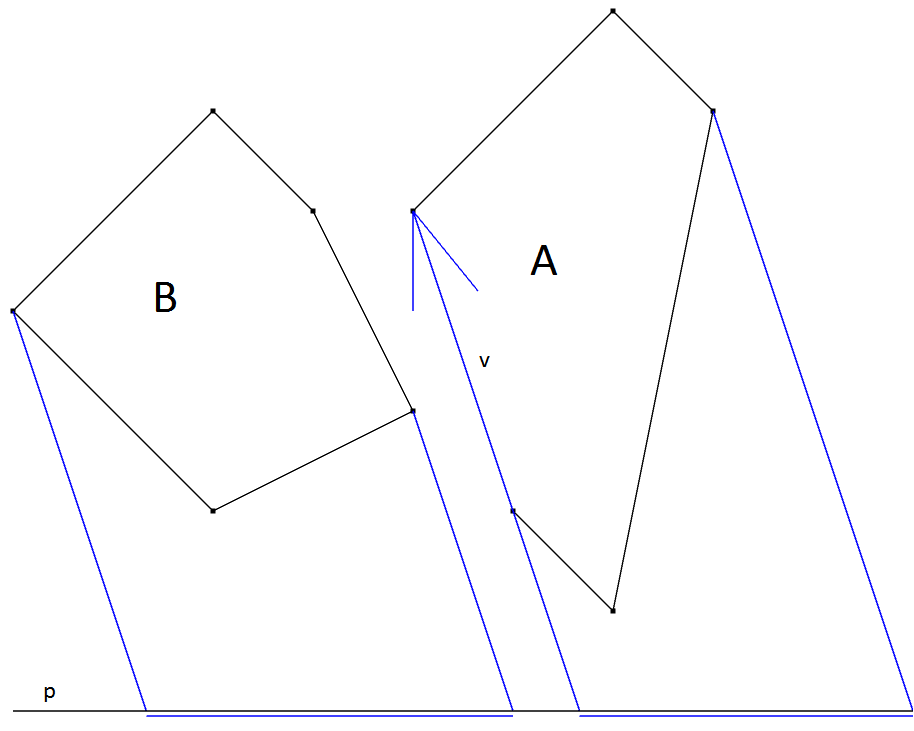
\includegraphics[width=\textwidth]{collission_separating_planes}
	\caption{Przykład wykrywania kolizji metodą płaszczyzn oddzielających, }
	\label{separating_planes}
\end{figure}

Jak widać na obrazku \ref{separating_planes}, obiekty A i B mają płaszczyznę oddzielającą równoległą do $v$, ponieważ ich rzuty na prostą $p$ nie pokrywają się. Dla A i C żadna płaszczyzna równoległa do $v$ nie oddziela tych obiektów, w kolejnym cyklu pętli jednak zostałaby znaleziona taka prosta, równoległa do następnego boku wielokąta A.
